% Options for packages loaded elsewhere
\PassOptionsToPackage{unicode}{hyperref}
\PassOptionsToPackage{hyphens}{url}
\documentclass[
]{article}
\usepackage{xcolor}
\usepackage[margin=1in]{geometry}
\usepackage{amsmath,amssymb}
\setcounter{secnumdepth}{-\maxdimen} % remove section numbering
\usepackage{iftex}
\ifPDFTeX
  \usepackage[T1]{fontenc}
  \usepackage[utf8]{inputenc}
  \usepackage{textcomp} % provide euro and other symbols
\else % if luatex or xetex
  \usepackage{unicode-math} % this also loads fontspec
  \defaultfontfeatures{Scale=MatchLowercase}
  \defaultfontfeatures[\rmfamily]{Ligatures=TeX,Scale=1}
\fi
\usepackage{lmodern}
\ifPDFTeX\else
  % xetex/luatex font selection
\fi
% Use upquote if available, for straight quotes in verbatim environments
\IfFileExists{upquote.sty}{\usepackage{upquote}}{}
\IfFileExists{microtype.sty}{% use microtype if available
  \usepackage[]{microtype}
  \UseMicrotypeSet[protrusion]{basicmath} % disable protrusion for tt fonts
}{}
\makeatletter
\@ifundefined{KOMAClassName}{% if non-KOMA class
  \IfFileExists{parskip.sty}{%
    \usepackage{parskip}
  }{% else
    \setlength{\parindent}{0pt}
    \setlength{\parskip}{6pt plus 2pt minus 1pt}}
}{% if KOMA class
  \KOMAoptions{parskip=half}}
\makeatother
\usepackage{graphicx}
\makeatletter
\newsavebox\pandoc@box
\newcommand*\pandocbounded[1]{% scales image to fit in text height/width
  \sbox\pandoc@box{#1}%
  \Gscale@div\@tempa{\textheight}{\dimexpr\ht\pandoc@box+\dp\pandoc@box\relax}%
  \Gscale@div\@tempb{\linewidth}{\wd\pandoc@box}%
  \ifdim\@tempb\p@<\@tempa\p@\let\@tempa\@tempb\fi% select the smaller of both
  \ifdim\@tempa\p@<\p@\scalebox{\@tempa}{\usebox\pandoc@box}%
  \else\usebox{\pandoc@box}%
  \fi%
}
% Set default figure placement to htbp
\def\fps@figure{htbp}
\makeatother
\setlength{\emergencystretch}{3em} % prevent overfull lines
\providecommand{\tightlist}{%
  \setlength{\itemsep}{0pt}\setlength{\parskip}{0pt}}
\usepackage{bookmark}
\IfFileExists{xurl.sty}{\usepackage{xurl}}{} % add URL line breaks if available
\urlstyle{same}
\hypersetup{
  pdftitle={Antra užduotis},
  pdfauthor={Skaistė Bartkutė, Viktorija Ramonaitė},
  hidelinks,
  pdfcreator={LaTeX via pandoc}}

\title{Antra užduotis}
\author{Skaistė Bartkutė, Viktorija Ramonaitė}
\date{2026-04-27}

\begin{document}
\maketitle

\subsection{1. Grupių palyginimas naudojant statistinį
testą.}\label{grupiux173-palyginimas-naudojant-statistinux12f-testux105.}

\textbf{Metodas}: pasirinktos tiriamųjų grupės prieš tyrimo intervenciją
(mėginiai paimti nuliniame laiko taške - T0) ir po tyrimo intervencijos
(laiko taškas - T18). Kadangi kiekvieno tiriamojo mėginiai sudaro
atitinkamas poras pagal paėmimo laikus, statistiniams testams
pasirinktas suporuotų mėginių (`paired') variantas. Kiekvienai CpG
pozicijai buvo apskaičiuota p vertė dviem statistiniais testais:
Studento t testu bei Vilkoksono testu. Gautų p verčių rinkiniams atlikta
FDR korekcija. Apskaičiuoti efekto dydžiai grupių vidurkių skirtumais
(kiekvienai CpG pozicijai).

\subsection{2. Patikimiausių skirtumų
profiliai.}\label{patikimiausiux173-skirtumux173-profiliai.}

\textbf{Metodas}: pagal atliktus abu statistinius testus atrinktos 10
CpG pozicijų su mažiausiomis p vertėmis (pagal kiekvieną testą
atskirai). Kiekvienai šiai CpG pozicijai iš T testo nubraižytas boxplot
ir DNR modifikacijos įverčių išsibarstymas. Taip pat nubraižyti
papildomi boxplots CpG pozicijoms, reikšmingoms pagal Vilkoksono testą,
kurios nepateko į T testo 10 reikšmingiausių pozicijų.

Pagal T testą gautos reikšmingiausios CpG pozicijos (nuo mažiausios p
vertės eilės tvarka): cg26210521, cg10992198, cg16872172, cg13315471,
cg07769732, cg27481720, cg01522525, cg10509965, cg20903764, cg04272309.

Pagal Vilkoksono testą gautos reikšmingiausios CpG pozicijos (nuo
mažiausios p vertės eilės tvarka): cg26210521, cg16872172, cg10992198,
cg13315471, cg01522525, cg17376730, cg27481720, cg09145071, cg20903764,
cg02364038.

Iš viso pagal abu testus sutampa 7 CpG pozicijos: cg26210521,
cg10992198, cg13315471, cg27481720, cg01522525, cg20903764.

\begin{center}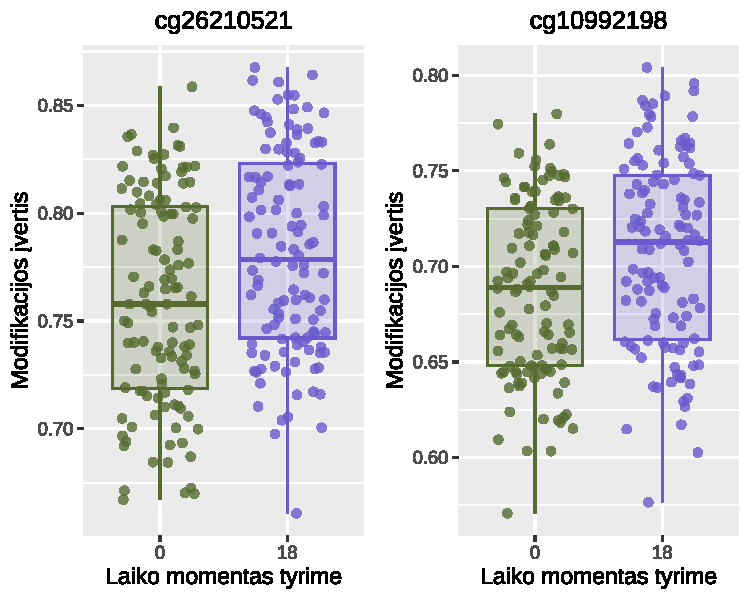
\includegraphics{Ataskaita_task2_files/figure-latex/significant-1} \end{center}

cg2610521 modifikacijos įverčių vidurkis po intervencijos pakyla nuo
apytiksliai 0.76 iki 0.77. Grupėje T18 matoma labiau nutolusi išskirtis
ties 0.66.

cg10992198 modifikacijos įverčių vidurkis pakyla nuo apytiksliai 0.69
iki 0.715. Grupėse T0 ir T18 taip pat pastebimos labiau nutolusios
išskirtys ties 0.56-0.57 lygiu.

\begin{center}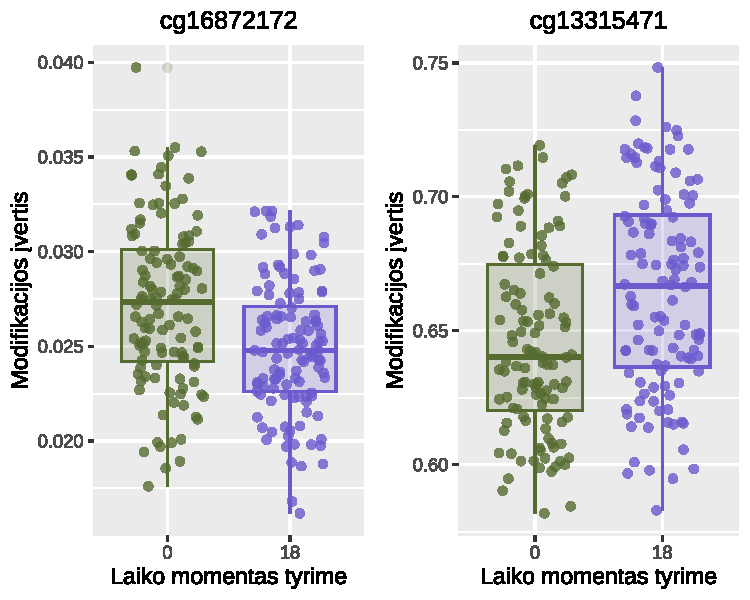
\includegraphics{Ataskaita_task2_files/figure-latex/p3p4-1} \end{center}

cg16872172 modifikacijos įverčių vidurkis po intervencijos sumažėja nuo
apytiksliai 0.027 iki 0.025. Pastebima labiausiai nutolusi išskirtis T0
grupėje ties 0.04 modifikacijos įverčio lygiu.

cg13315471 modifikacijos įverčių vidurkis po intervencijos pakyla nuo
apytiksliai 0.64 iki 0.67. T18 grupėje matosi išskirtys ties 0.575 ir
0.75 įverčių lygiais.

\begin{center}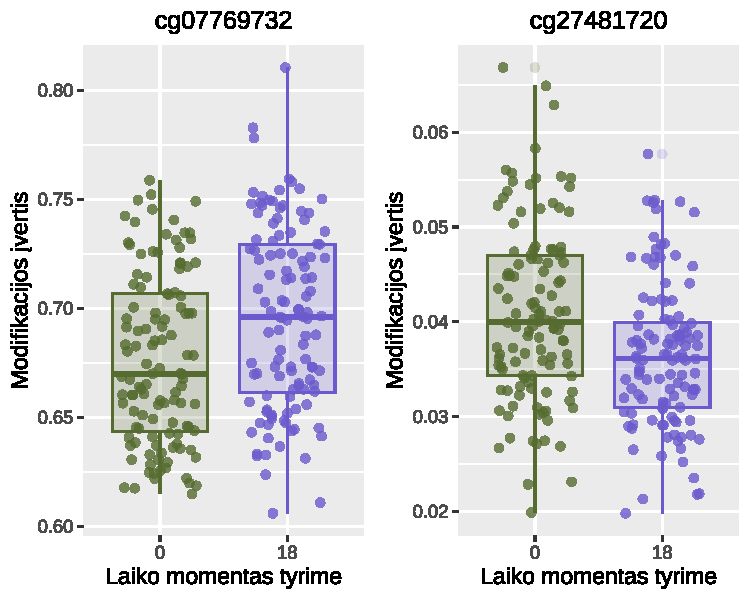
\includegraphics{Ataskaita_task2_files/figure-latex/p5p6-1} \end{center}

cg07769732 modifkacijos įverčių vidurkis po intervencijos pakyla nuo
apytiksliai 0.67 iki 0.7. Grupė T18 turi platų įverčių diapazoną su
labiau matomomis išskirtimis ties 0.6 ir 0.81 ribomis.

cg27481720 modifikacijos įverčių vidurkis po intervencijos sumažėja nuo
apytiksliai 0.04 iki 0.036. Grupė T0 turi platų įverčių diapazoną su
išskirtimis ties 0.02 ir 0.065 lygiais, o T0 grupėje matoma toliausiai
nutolusi išskirtis ties 0.057 lygiu.

\begin{center}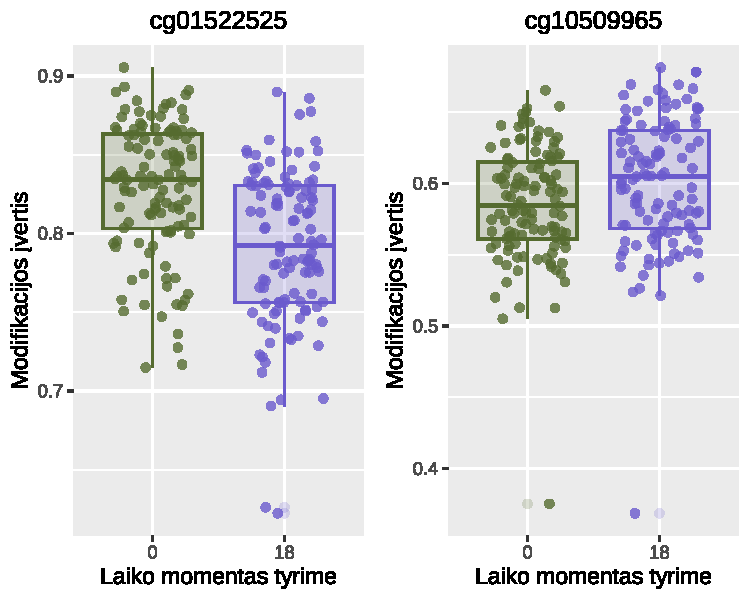
\includegraphics{Ataskaita_task2_files/figure-latex/p7p8-1} \end{center}

cg01522525 modifikacijos įverčių vidurkis po intervencijos sumažėja nuo
apytiksliai 0.83 iki 0.79. Grupėje T18 matomos kelios ryškesnės
išskirtys ties 0.63 lygiu.

cg10509965 modifikacijos įverčių vidurkis po intervencijos pakyla nuo
apytiksliai 0.58 iki 0.61. Tiek grupėje T0, tiek T18 pastebimos tolimos
išskirtys ties 0.37 modifikacijos įverčio lygiu.

\begin{center}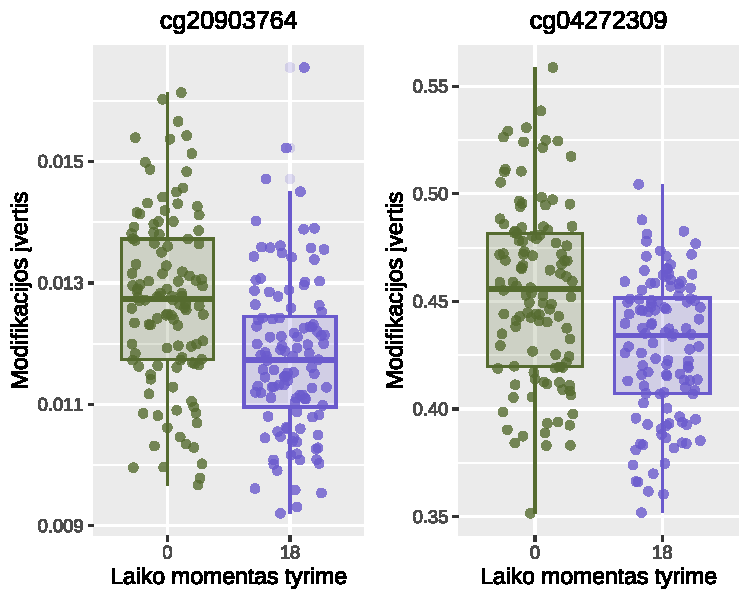
\includegraphics{Ataskaita_task2_files/figure-latex/p9p10-1} \end{center}

cg20903764 modifikacijos įverčių vidurkis po intervencijos sumažėja nuo
apytiksliai 0.0128 iki 0.0118. Įverčiai grupėse T0 ir T18 plačiai
išsibarstę, matoma išskirtis T18 grupėje 0.0165 lygiu.

cg04272309 modifikacijos įverčių vidurkis po intervencijos sumažėja nuo
apytiksliai 0.46 iki 0.44. Grupėje T0 matomos išskirtys ties 0.35 ir
0.56 modifikacijos įverčių lygiais.

CpG pozicijos, kuriose modifikacijos įvertis statistiškai reikšmingai
padidėjo po intervencijos: cg26210521, cg10992198, cg13315471,
cg07769732, cg10509965. CpG pozicijos, kuriose modifikacijos įvertis
statistiškai reikšmingai sumažėjo po intervencijos: cg16872172,
cg27481720, cg01522525, cg20903764, cg04272309.

Kitos trys CpG pozicijos iš Vilkoksono testo: cg17376730, cg09145071,
cg02364038.

\begin{center}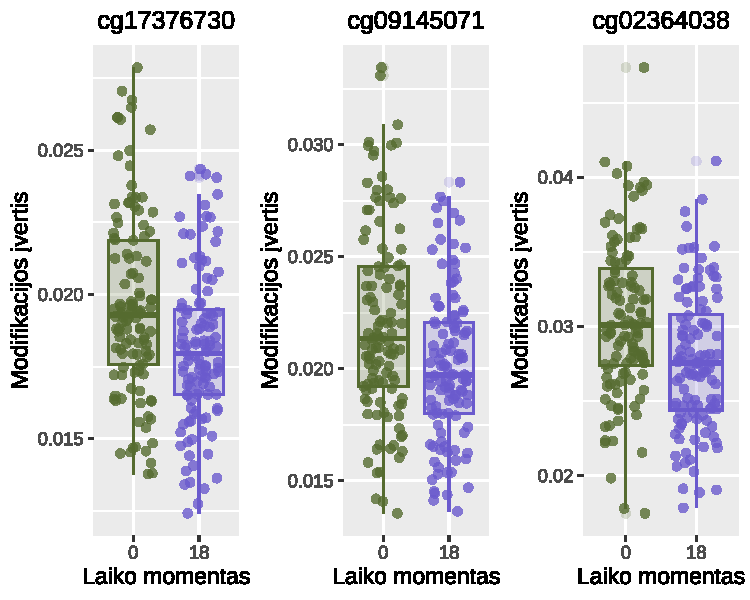
\includegraphics{Ataskaita_task2_files/figure-latex/wilcoxon-1} \end{center}

cg17376730 modifikacijos įverčių vidurkis po intervencijos sumažėja nuo
apytiksliai 0.019 iki 0.0175. Tiek T0, tiek T18 grupės diapazonai
platūs.

cg09145071 modifikacijos įverčių vidurkis po intervencijos sumažėja nuo
apytiksliai 0.022 iki 0.020. T0 grupėje matomos išskirtys ties 0.033
modifikacijos lygiu.

cg02364038 modifikacijos įverčių vidurkis po intervencijos sumažėja nuo
apytiksliai 0.030 iki 0.027. T0 grupėje matomos išskirtys ties 0.018 bei
0.048 modifikacijos lygiais, o T18 išskirtis ties 0.041 įverčiu.

Visų šių modifikacijų įverčiai statistiškai reikšmingai sumažėję:
cg17376730, cg09145071, cg02364038.

\subsection{3. P verčių
histogramos.}\label{p-verux10diux173-histogramos.}

\textbf{Metodas}: histogramose pavaizduojamas p verčių pasiskirstymas
(intervalais po 0.01) ir apskaičiuotas statistiškai patikimų (p
\textless{} 0.05) CpG pozicijų (pagal modifikacijos įverčių pasikeitimą)
kiekis.

\begin{center}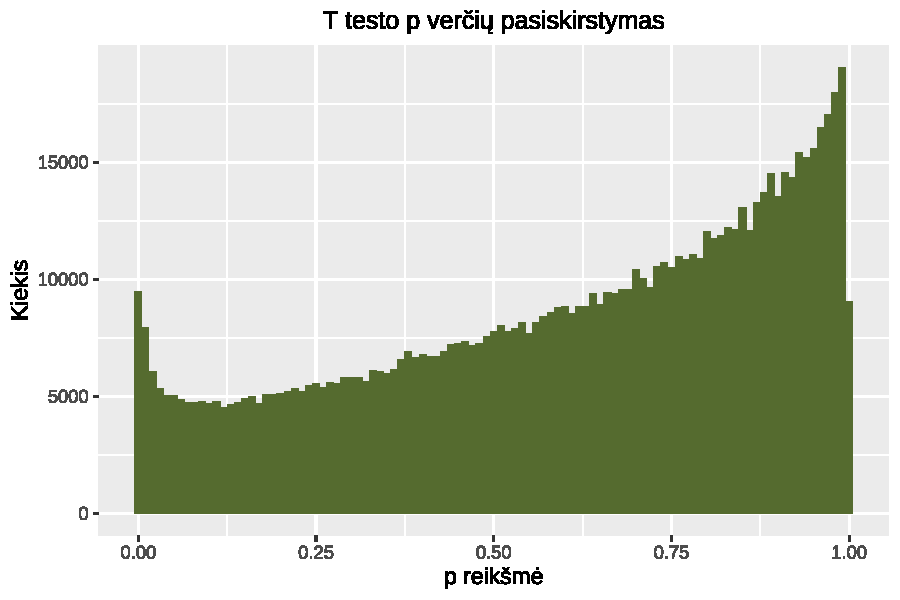
\includegraphics{Ataskaita_task2_files/figure-latex/ttest_histogram-1} \end{center}

Pagal T testą matyti, kad tik nedidelė dalis CpG pozicijų yra
statistiškai reikšmingai besiskiriančios prieš ir po intervencijos:
39395 iš 865859 (4.2\%). Daugiausiai p verčių pasislinkusios į 1.0
vertės pusę (neturi statistinio reikšmingumo).

\begin{center}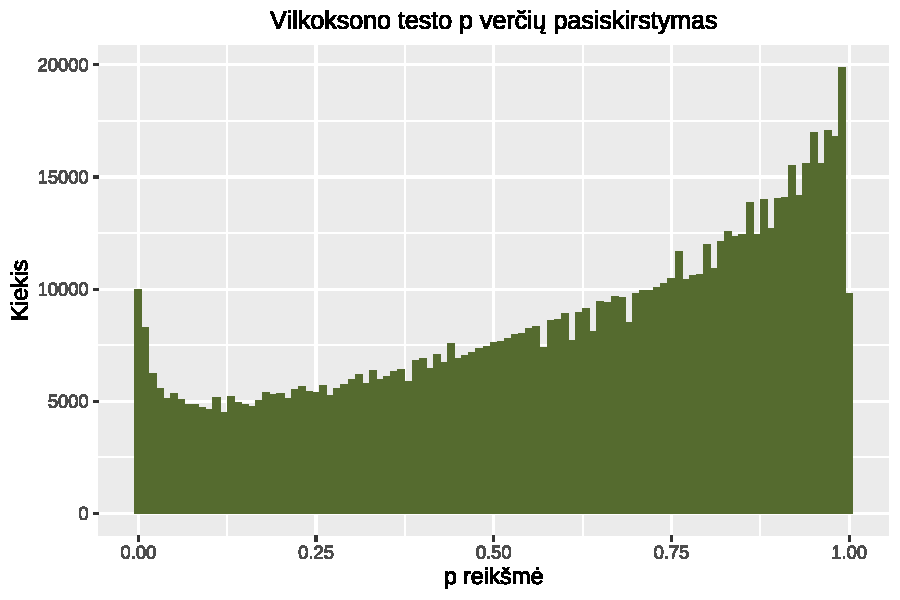
\includegraphics{Ataskaita_task2_files/figure-latex/wilcoxon_histogram-1} \end{center}

Su Vilkoksono testu situacija panaši kaip su t testu: tik nedidelė dalis
CpG pozicijų yra statistiškai reikšmingos (37902 arba 4.38\%), daug CpG
pozicijų turi didelę p vertę, rodančią, jog jose reikšmingo skirtumo
modifikacijose įverčiuose prieš ir po intervencijos nepastebima.

\subsection{4. Volcano grafikas.}\label{volcano-grafikas.}

\textbf{Metodas}: volcano grafike pavaizduotas vidurkių skirtumas (T18 -
T0) x ašyje ir -log10 transformuota FDR koreguota p vertė y ašyje. CpG
pozicijos suskirstytos į tris kategorijas: hipermetilinta (p \textless{}
0.05 ir vidurkių skirtumas \textgreater{} 0.01), hipometilinta (p
\textless{} 0.05 ir vidurkių skirtumas \textless{} -0.01) ir
nereikšminga (visos likusios). Punktyrinės linijos žymi reikšmingumo
slenksčius: horizontali - p = 0.05, vertikalios - vidurkių skirtumo
±0.01 ribos.

\begin{center}\includegraphics{Ataskaita_task2_files/figure-latex/volcano-1} \end{center}

Volcano grafike matyti, kad didžioji dalis CpG pozicijų yra
nereikšmingos (pilki taškai, susikoncentravę centro apačioje).
Hipermetilintų (raudonų) CpG pozicijų pasiskirstymas dešinėje pusėje yra
platesnis nei hipometilintų (mėlynų) kairėje, kas rodo, kad intervencija
sukėlė kiek stipresnius metilinimo padidėjimo efektus. Reikšmingiausia
CpG pozicija (aukščiausias taškas, -log10(p) ≈ 12) priklauso
hipermetilintai grupei. Hipometilintoje grupėje taip pat pastebimi keli
taškai su aukštomis -log10(p) vertėmis (≈ 8--9). Grafike taip pat matoma
didelė pilkų taškų grupė tarp vertikalių slenksčių (vidurkių skirtumas
tarp -0.01 ir 0.01), kurios p vertės yra reikšmingos --- tai CpG
pozicijos su statistiškai patikimais, bet biologiškai mažais metilinimo
pokyčiais.

\subsection{5. Manhattan grafikas.}\label{manhattan-grafikas.}

\textbf{Metodas}: Manhattan grafike kiekvienai CpG pozicijai pavaizduota
-log10(p) vertė pagal jos genominę poziciją chromosomose. Naudotos FDR
koreguotos p vertės iš T testo. Horizontali raudona linija žymi
reikšmingumo slenkstį (p = 0.05). Papildomai nubraižytas atskiras
Manhattan grafikas 19 chromosomai, kuri pasižymėjo didžiausiu reikšmingų
CpG pozicijų tankiu.

\begin{center}\includegraphics{Ataskaita_task2_files/figure-latex/manhattan_whole-1} \end{center}

Manhattan grafike matyti, kad reikšmingų CpG pozicijų (virš raudonos
linijos, žyminčios p = 0.05) yra daug visose chromosomose. Reikšmingų
taškų pasiskirstymas tarp chromosomų yra gana tolygus, be ryškių lokusų.
Stipriausias signalas matomas 3 chromosomoje, kur vienas taškas pasiekia
-log10(p) ≈ 12.5.19 chromosoma išsiskiria didesniu reikšmingų taškų
tankiu viršutinėje grafiko dalyje (-log10(p) \textgreater{} 5), todėl ji
pasirinkta detalesnei analizei atskirame grafike. Bendrai grafike
nematyti vienos dominuojančios genominės srities --- intervencijos
efektas metilinimui yra pasiskirstęs panašiai per visą genomą.

\begin{center}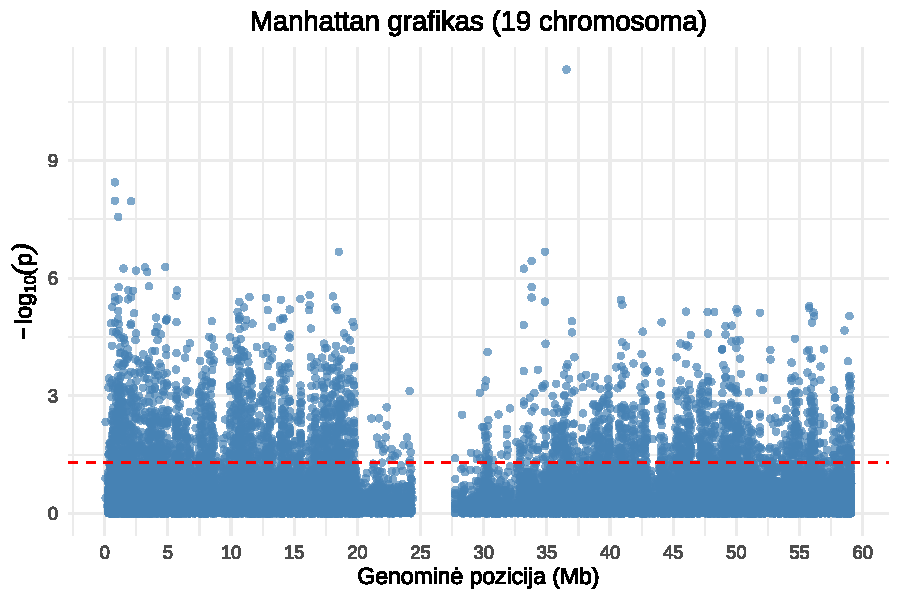
\includegraphics{Ataskaita_task2_files/figure-latex/manhattan_chromosome-1} \end{center}

19 chromosomoje reikšmingos CpG pozicijos (virš raudonos punktyrinės
linijos) pasiskirstę netolygiai. Matomi du aiškūs CpG pozicijų tankio
regionai: 0--25 Mb ir 28--60 Mb, tarp kurių (ties \textasciitilde25--27
Mb) pastebimas tarpas, kur nėra CpG pozicijų --- tai greičiausiai
atitinka 19 chromosomos centromero sritį, kurioje CpG beveik nėra.
Stipriausias signalas pasiekia -log10(p) ≈ 10. Kiti ryškesni signalai
(-log10(p) \textgreater{} 7) matomi chromosomos pradžioje. Pirmoje
chromosomos dalyje (0--20 Mb) reikšmingų taškų tankis atrodo didesnis
nei antroje (28--60 Mb), kur taškai labiau išsibarstę. Sritys su
padidėjusiu reikšmingų CpG pozicijų tankiu pastebimos visoje
chromosomoje --- šios sritys gali atitikti genų klasterius, kuriuose
intervencija sukėlė metilinimo pokyčius.

\subsection{6. GO analizė.}\label{go-analizux117.}

\textbf{Metodas}: CpG pozicijos, kurių FDR koreguota p vertė \textless{}
0.05, buvo padalintos į dvi grupes pagal metilinimo pokyčio kryptį:
hipermetilintą (T18 vidurkis \textgreater{} T0 vidurkis) ir
hipometilintą (T18 vidurkis \textless{} T0 vidurkis). Kiekvienai grupei
išrinkti unikalūs genų pavadinimai. Genų ontologijos (GO) analizė
atlikta naudojant GOrilla internetinį įrankį, pateikiant tikslinį gautą
sąrašą ir grafikus.

\textbf{Grafikai}: Dėl didelių grafkų, grafikai neįdėti į apžvalgą, juos
peržiūrėti galima github puslapyje:
\url{https://github.com/LunaMoonax/Yaskolka_Biomedicine_analysis}

Grafikų ir rezultatų pavadinimai githube: GOrilla results
hyper\_files/top.html - visi rezultatai hipermetilintai grupei (yra tiek
grafikas, tiek lentelė) GOrilla results hypo\_files/top.html - visi
rezultatai hipometilintai grupei (yra tiek grafikas, tiek lentelė)
p\_values.png - spalvinė legenda p reikšmių. Kuo raudonesnė - tuo
reikšmingesnė. GOPROCESS\_hyper\_process.png - hipermetilintos grupės GO
analizė biologinių procesų grafikas. GOFUNCTION\_hyper\_function.png -
hipermetilintos grupės GO analizė molekulinės funkcijų grafikas.
GOCOMPONENT\_hyper\_component.png - hipermetilintos grupės GO analizė
ląstelės komponentų grafikas. GOPROCESS\_hypo\_process.png -
hipometilintos grupės GO analizė biologinių procesų grafikas.
GOFUNCTION\_hypo\_function.png - hipometilintos grupės GO analizė
molekulinės funkcijų grafikas. GOCOMPONENT\_hypo\_component.png -
hipometilintos grupės GO analizė ląstelės komponentų grafikas.

\textbf{Išvados}: Biologinis procesas (Process): Hipermetilinti genai:
stipriausiai praturtinti procesai susiję su ląstelių adhezija, vystymusi
ir nervų sistemos reguliacija --- neuronų projekcijų valdymu, aksonų
orientavimu (daugiausiai raudonų nuspalvintų procesų). Taip pat
reikšmingai praturtinti signalizacijos reguliacijos, fosforilinimo ir
GTPazės aktyvumo reguliacijos procesai. Hipometilinti genai:
vizualizacija labai tanki su daugybe raudonų funkcijų, kas rodo, kad
hipometilintų genų grupė paveikia platesnį biologinių procesų spektrą.
Paraudonėjo daug funkcijų susijusių su metaboliniais keliais ir
funkcijomis, reguliacijos mechanizmai, ląstelės lokalizacija. Tai gali
reikšti, kad metilinimo sumažėjimas po intervencijos apima daugiau
skirtingų biologinių kelių, įskaitant metabolinius, reguliacinius ir
signalizacijos procesus.

Molekulinė funkcija (Function): Hipermetilinti genai: praturtintos
molekulinės funkcijos apima kinazės aktyvumą, transferazės aktyvumą,
jonų kanalų aktyvumą (ypač kalcio ir kalio kanalai), receptorių surišimą
bei transkripcijos faktorių surišimą. Daug raudonų funkcijų susiję su
baltymų fosforilinimu ir signaliniu perdavimu per membraną.
Hipometilinti genai: matoma panašios funkcijos nuspalvintos raudonai,
kaip ir hipermetilintų genų, bet taip pat yra ir daugiau. Praturtintos
funkcijos apima DNR surišimą, transkripcijos reguliatorinį aktyvumą,
katalizinį aktyvumą ir transporterio aktyvumą, kas rodo platų genų
ekspresijos reguliacijos poveikį.

Ląstelinis komponentas (Component): Hipermetilinti genai: stipriausiai
praturtinti komponentai susiję su sinapsėmis (glutamatergine,
GABAergine, Schaffer kolateraline sinapse), ląstelės jungtimis,
plazminės membranos komponentais, citoskeletu ir tarpląstelinės matricos
struktūromis. Tai dera su biologinio proceso rezultatais, kur dominuoja
adhezijos ir nervų sistemos terminai. Hipometilinti genai: praturtinti
ląsteliniai komponentai apima membranos dalis, intrinsines membranos
komponentus, branduolio dalis ir chromatino struktūras. Skirtingai nuo
hipermetilintų genų, čia labiau akcentuojami vidiniai ląsteliniai
komponentai, o ne tarpląsteliniai kontaktai.

Bendra GO analizės išvada: GO analizė atskleidė, kad hipermetilinti ir
hipometilinti genai paveikia skirtingus biologinius kelius.
Hipermetilintų genų grupė labiau susijusi su ląstelių sąveika, adhezija
ir sinapsine signalizacija, o hipometilintų genų grupė --- su
platesniais metaboliniais bei genų ekspresijos reguliacijos procesais.
Abiejose grupėse pastebimas stiprus nervų sistemos ir signalizacijos
kelių praturtinimas, kas gali rodyti intervencijos poveikį neuronų
mechanizmams.

\subsection{7. Stipriausių efekto dydžių apžvalginė
analizė}\label{stipriausiux173-efekto-dydux17eiux173-apux17evalginux117-analizux117}

Vienas iš būdų apibūdinti efekto dydį - Cohen's d.~Jis apibrėžia efekto
dydį kaip vidurkių skirtumą standartinio nuokrypio vienetais. Kitas
efekto dydis: r (rank-biserial) - koreliacija apskaičiuojama suskirstant
grupes į rangus panašiai kaip Wilcoxon suporuotų grupių testu.

\textbf{Metodas}: apskaičiuoti Cohen's d ir rank-biserial efekto dydžiai
CpG pozicijoms (lyginant T0 ir T18 laiko taškus). Atsirinktos
statistiškai reikšmingos CpG pozicijos (p\textless0.05). Atlikta atranka
pagal vidutinį efekto dydžio slenkstį abiems efekto dydžių tipams: 0.5.
Taip pat atrinktos CpG pozicijos, kurių vidurkių skirtumas (mean
difference) didesnis negu 0.1 (trečia efekto dydžių grupė). Toks
skirtumas parinktas atsižvelgiant į tai, kad buvo norima rasti daugiau
sutampančių CpG pozicijų tarp skirtingų efekto dydžių grupių.

Cohen's d ir rank biserial vidutinių ir stiprių efekto dydžių sąrašams
buvo rastos 306 bendros CpG pozicijos. Pagal vidurkių skirtumo efekto
dydžius ir Cohens'd efekto dydžius bendros buvo 124 CpG pozicijos, o
pagal vidurkių skirtumo efekto dydžius ir rank biserial efekto dydžius
bendros 359 CpG pozicijos.

\textbf{Metodas}: turint pagal efekto dydžius atrinkas CpG pozicijas
stulpelinėse diagramose buvo pavaizduotas jų pasiskirstymas (CpG
pozicijų kiekis) atitinkamuose regionuose (salos, atviros jūros sritys,
šelfai ir pakrantės). Kiekvienam efekto dydžio tipui sudaroma atskira
stulpelinė diagrama.

\begin{center}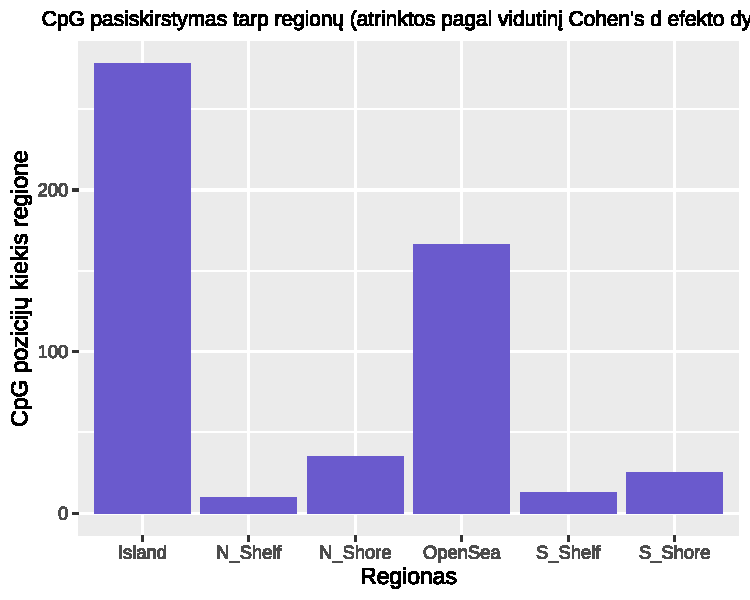
\includegraphics{Ataskaita_task2_files/figure-latex/islands-1} \end{center}

\begin{center}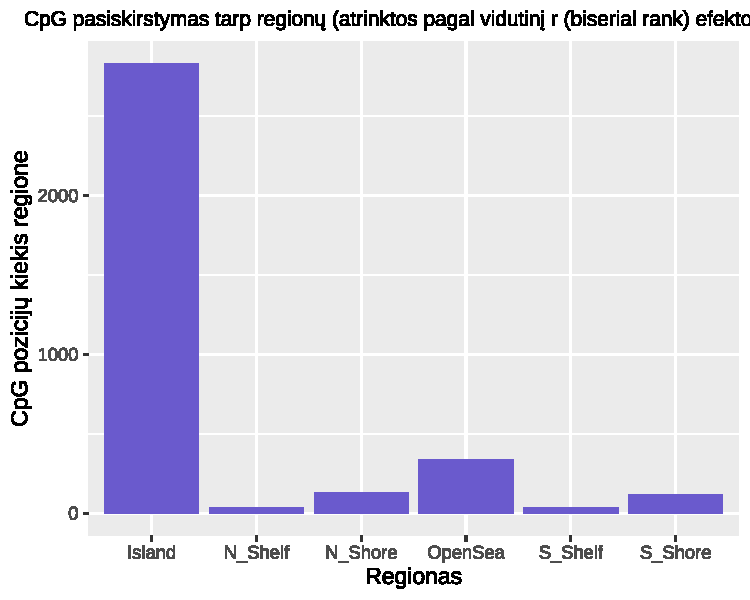
\includegraphics{Ataskaita_task2_files/figure-latex/islands-2} \end{center}

\begin{center}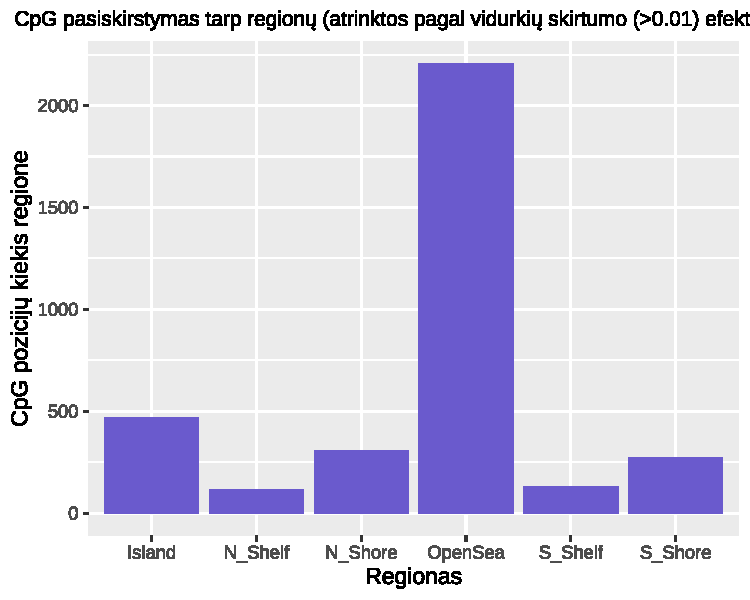
\includegraphics{Ataskaita_task2_files/figure-latex/islands-3} \end{center}

Pagal vidutinį ir stiprų Cohen's d efekto dydį daugiausiai CpG pozicijų
yra salose ir perpus mažiau atviros jūros regione ir pavieniai atvejai
kitose srityse. Pagal vidutinį ir stiprų rank biserial efekto dydį
beveik visos CpG pozicijos yra salose ir lyginant daug mažiau kituose
regionuose. Didesni efekto dydžiai salose galėtų reikšti genų
įjungimą/nutildymą. Reiktų atsižvelgti į tai, kad CpG pozicijų sąrašai
ne vienodo ilgio: Cohens' d - 527 CpG pozicijos, rank biserial - 3483, o
pagal vidurkių skirtumą - 3501. Vidurkių skirtumo efekto dydis rodo
kitokią tendenciją - daugiausiai CpG pozicijų atviros jūrose regionuose,
t.y. intergeniniuose regionuose arba pačių genų koduojančiose srityse,
kas galbūt nebūtinai susiję su genų nutildymu ar įjungimu. Tokie
skirtumai gali atsirasti dėl to, kad Cohend's d ir rank biserial yra
standartizuoti efekto dydžiai, o vidurkių skirtumas - ne.

\textbf{Metodas}: pagal kiekvieno efekto dydžio tipą atrinkti 10 CpG
pozicijų su stipriausiais efekto dydžiais. Šioms grupėms sudaryti
heatmap'ai.

Tarp Cohen's d ir rank biserial grupių sutapusi CpG pozicija -
cg01522525. Tarp vidurkių skirtumo ir Cohen's d grupių dar sutapo
cg05001044 bei cg22519184, o tarp vidurkių skirtumo ir rank biserial
nebuvo sutapusių CpG pozicijų.

\subsection{Heatmap, kuriame CpG pozicijos atrinktos pagal didžiausius
Cohen's d efekto dydžius
(top10).}\label{heatmap-kuriame-cpg-pozicijos-atrinktos-pagal-didux17eiausius-cohens-d-efekto-dydux17eius-top10.}

\begin{center}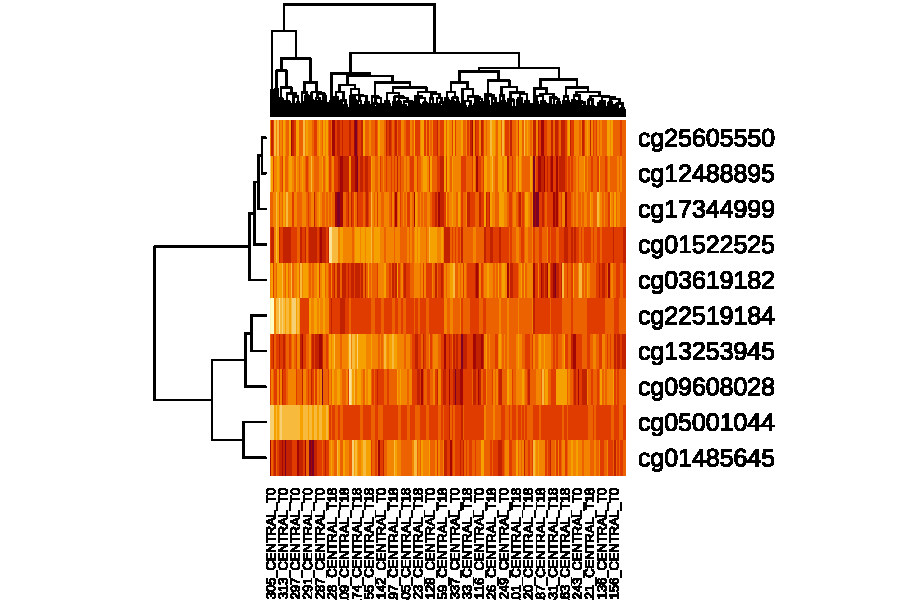
\includegraphics{Ataskaita_task2_files/figure-latex/heatmap1-1} \end{center}

Šiame heatmap'e sunkiau įžvelgti susigrupavimus pagal spalvas, bet ties
kiekviena CpG pozicija matoma daug skirtingų spalvų intensyvumų, kas
reikštų skirtingus metilinimo įverčius ir didesnius efekto dydžius.

\subsection{Heatmap, kuriame CpG pozicijos atrinktos pagal didžiausius
rank biserial efekto dydžius
(top10).}\label{heatmap-kuriame-cpg-pozicijos-atrinktos-pagal-didux17eiausius-rank-biserial-efekto-dydux17eius-top10.}

\begin{center}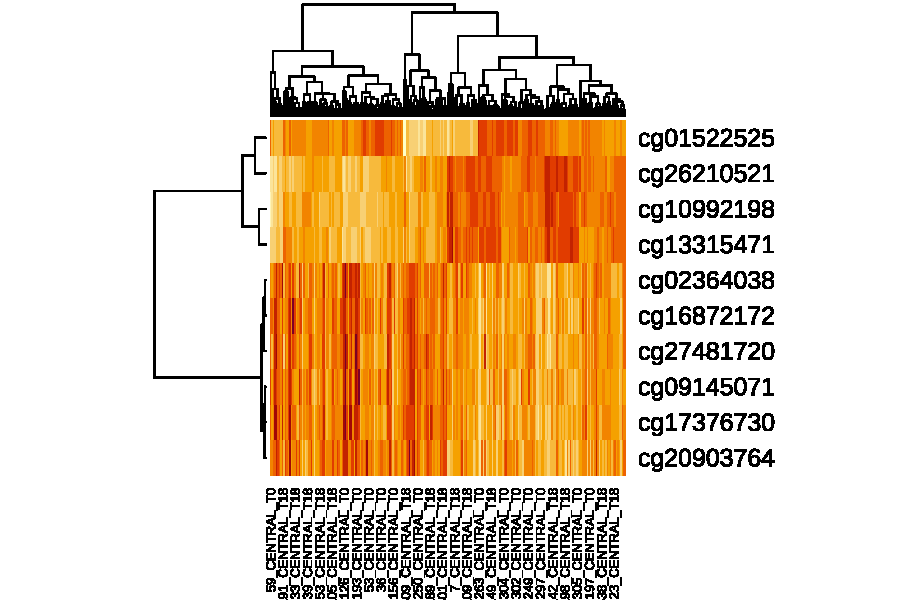
\includegraphics{Ataskaita_task2_files/figure-latex/heatmap2-1} \end{center}

Šiame heatmap labiau matomas atsiskyrimas tarp modifikacijos įverčių
padidėjimo/sumažėjimo. Pavyzdžiui, cg26210521 iš ankstesnio grafiko
susijęs su modifikacijos įverčių vidurkio padidėjimu (kairėje pusėje
silpnesnis metilinimas, dėšinėje stipresnis). Apatinė heatmap dalis
labiau susijusi su modifikacijos įverčių vidurkių sumažėjimu (pvz.
cg02364038, cg16872172 iš praeitų grafikų). Kairėje pusėje labiau
pastebimi didesni įverčiai, o dešinėje mažesni. Dėl tokių skirtumų
atsiranda dideli efekto dydžiai.

\subsection{Heatmap, kuriame CpG pozicijos atrinktos pagal didžiausius
vidurkių skirtumus tarp grupių
(top10).}\label{heatmap-kuriame-cpg-pozicijos-atrinktos-pagal-didux17eiausius-vidurkiux173-skirtumus-tarp-grupiux173-top10.}

\begin{center}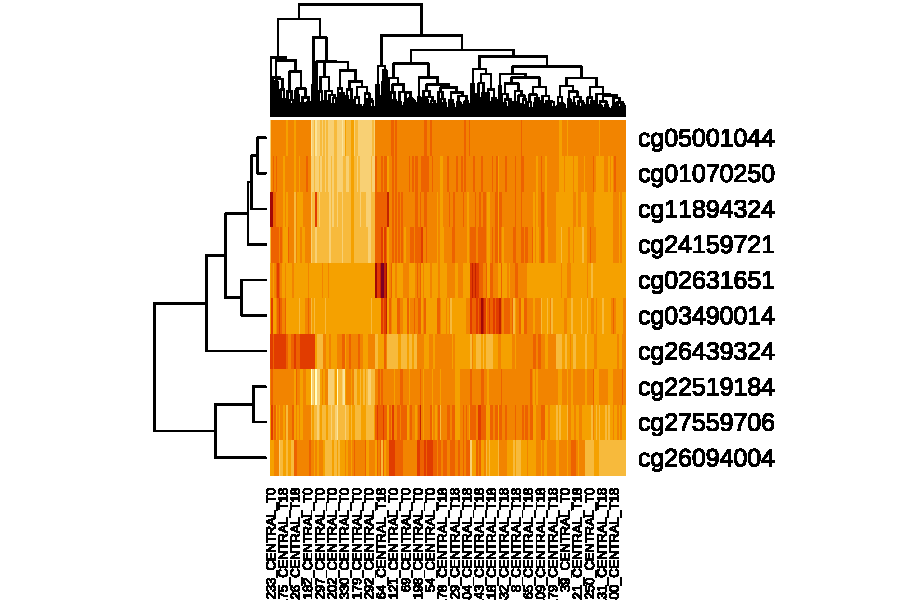
\includegraphics{Ataskaita_task2_files/figure-latex/heatmap3-1} \end{center}

Šiame heatmap CpG pozicijų modifikacijos įverčiai neturi tokių didelių
modifikacijos skirtumų (vientisesnės spalvos). Išskirčių matoma
cg02631651 ir cg03490014, cg26439324, kur yra aukštesnių modifikacijos
įverčių. Tačiau skirtumai tarp grupių pakankami gauti didelius vidurkių
skirtumus. Galbūt CpG pozicijų nesutapimas su kitų efektų dydžių
grupėmis atsiranda dėl to, kad kitų efektų dydžių CpG pozicijų
metilinimo skirtumai, nors ir didesni, kompensuoja vienas kitą, ir gali
nepatekti į top 10 didžiausių vidurkių skirtumų sąrašą.

\end{document}
